%!Mode:: "TeX:UTF-8"
\documentclass[a4paper,12pts]{article}

\usepackage[polish]{babel}
\usepackage[utf8]{inputenc}
\usepackage{fontspec}
\setmainfont{Calibri}

\linespread{1.15}

\usepackage{caption}
\captionsetup{%
	font={footnotesize},
	labelfont={bf}
}

\usepackage{anysize}
\usepackage{geometry}

\usepackage{graphicx}


% Plik szablonowy do wykorzystania pózniej - nie zmieniaj go!
% Użwyaj kompilatora XELATEX

\begin{document}
	\thispagestyle{empty}
	\begin{flushleft}
		Wydział Elektrotechniki, Automatyki, Informatyki i Inżynierii Biomedycznej \\
		Informatyka, rok II \\
		Zespół numer 3 \\
		Piotr Kucharski \\
		Dominik Zabłotny \\
		\vspace*{\fill}
		%-----------NUMER CWICZENIA--------%
		{\large \textbf{Sprawozdanie z ćwiczenia nr 29} } \\
		%-----------TEMAT ĆWICZENIA--------%
		Fale podłóżne w ciałach stałych.	
		\vfill	
		%-----------DATA-------------%
		18 października 2017r
	\end{flushleft}
	
	\newpage
	
%--------------------------------------------------------------------------------------------------------------

\section{Wstęp}

\subsection{Cele ćwiczenia}
Celem ćwiczenia jest wyznaczenie modułu Younga dla prętów różnych materiałów na podstawie pomiarów ich częstotliwości harmonicznych.

\subsection{Wprowadzenie teoretyczne}
\subsubsection{Fala podłużna}
Fala podłóżna jest to fala powstająca przez gwałtowne wychylenie ciała z położenia równowagi oraz dalszemu jego drganiu aż do momentu odzyskania równowagi. Szybkość rozchodzenia się tej fali zależy od bezwładności i sprężystości ciała.

\subsection{Fala stojąca}
Fala, której grzbiety i doliny nie przemieszaczją się. Powstaje na skutek interferencji dwóch takich samych fal podłużnych, w przypadku pręta przez odbicie fali o przeciwległy koniec do uderzonego młotkiem. Falę stojącą określa się równaniem:
\begin{equation}
y = 2A \sin kx
\end{equation}

\subsubsection{Moduł Younga}
Wielkość charakteryzującą sprężystość materiału, będąca jego integralną częścią nazywamy modułem Younga oraz oznaczamy go jako $E$. Ogólny wzór na moduł Younga określa się jako stosunek naprężenia $\sigma$ do względnego odkszałcenia liniowego $\varepsilon$ materiału:
\begin{equation}
E = \frac{\sigma}{\varepsilon}
\end{equation}
Po uwzględnieniu, że ćwiczenie przeprowadzane jest na prętach różnych materiałów, interferencji fali padającej i fali odbitej oraz prawa Hooke'a uzyskujemy wzór:
\begin{equation}
E = 4 \rho l^2 f^2
\end{equation}
gdzie $\rho$ to gęstość materiału, $l$ - odległość między węzłami fali oraz $f$ częstotliwość fali podłużnej. Tego wzoru będziemy używać do wykonania ćwiczenia.


\subsubsection{Analiza Fouriera}
Jest to proces badania drgań harmonicznych, polega na przedstawieniu funkcji okresowej w postaci nieskończonego szeregu trygonometrycznego (szeregu Fouriera). W naszym doświadczeniu wykorzystujemy program Zelscope, który realizuje algorytm FFT pozwalający na szybkie obliczenie transformaty Fouriera i przedstawia ją jako widmo fali na ekranie (analogicznie do oscyloskopu znanego z elektroniki). Będziemy odczytywać kolejne wartości drgań harmonicznych z ekranu.

\subsection{Układ pomiarowy}
Układ pomiarowy składa się z komputera z zainstalowanym oprogramowaniem Zelscope, mikrofonu podłączonego do komuptera, długich prętów wykonanych z różnych materiałów zawieszonych na nitkach w dwóch miejscach. Do wprawienia ciał w drgania użyjemy młotka, do pomiaru długości prętów użyjemy miary milimetrowej zwijanej, do pomiaru masy prętów użyjemy wagi elektronicznej firmy RAWAG model WTB 200 oraz do zmierzenia grubości materiałów w celu wyznaczenia ich objętości użyjemy suwmiarki.

\begin{figure}[!h]
	\centering
	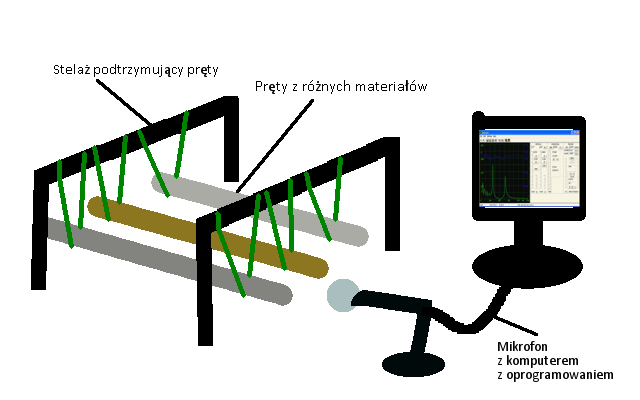
\includegraphics[scale=0.5]{schemat}
	\caption{Schemat układu pomiarowego}
	\label{schematUkladu}
\end{figure}

%--------------------------------------------------------------------------------------------------------------

\section{Wykonanie ćwiczenia}
Wykonanie ćwiczenia dzieli się na dwa kroki stosowane dla każdego badanego pręta oraz jednej wspólnej analizy wyników.
\subsection{Pomiary specyfikacji prętów}
\begin{itemize}
	\item Pomiar długości pręta za pomocą miary zwijanej.
	\item Pomiar grubości pręta za pomocą suwmiarki (w przypadku otwartego walca mierzymy promień zewnętrzny i wewnętrzny).
	\item Zważenie pręta w najlepszy możliwy sposób za pomocą wagi elektronicznej.
	\item Zapisanie wyników o danym ciele do tabeli.
\end{itemize}
\newpage
\subsection{Pomiar częstotliwości harmonicznych}
\begin{itemize}
	\item Osadzenie preta w niciach zamontowanych do stelaża.
	\item Przybliżenie mikrofonu do badanego pręta.
	\item Uderzenie młotkiem w pręt aby wprawić go w drganie.
	\item Zamrożenie odczytu programu Zelscope w momencie najlepszej widoczności widma fal harmonicznych.
	\item Odczyt sześciu pierwszych harmonicznych (jeżeli taką ilość udało się zaobserwować).
\end{itemize}
W przypadku niejednoznacznego odczytu częstotliwości harmonicznych nalezy powtórzyć pomiar.

\subsection{Oblicznanie koniecznych wartości}
Z zapisanych danych pomiarowych należy obliczyć gęstość ciała daną wzorem:
\begin{equation}
\rho = \frac{m}{V}
\end{equation}
gdzie $m$ to zmierzona masa ciała oraz $V$ to objętość ciała obliczona odpowiednio dla każdego pręta z odpowiednich wielkości. Pręty są różnymi figurami przestrzennymi, przez wykorzystujemy odpowiedni wzór dla:
\begin{itemize}
	\item walca o promieniu podstawy $r$ oraz wysokości $h$
	\begin{equation}
	V = \pi r^2 h
	\end{equation}
	
	\item prostopadłościanu prawidłowego czworokątnego o krawędzi podstawy $a$ oraz wysokości $h$
	\begin{equation}
	V = a^2 h
	\end{equation}
	
	\item otwartego walca o promieniu zewnętrznym podstawy $R$, promieniu wewnętrznym podstawy $r$ oraz wysokości $h$
	\begin{equation}
	V = \pi (R^2 - r^2) h
	\end{equation}
\end{itemize}
Do oblicznia długości fali $\lambda$ zastosujemy zależność stosunku długości pręta $L$ do numeru harmonicznej fali $n$:
\begin{equation}
\lambda = \frac{2L}{n}
\end{equation}
Odległość $l$ między węzłami fali stojącej stanowi połowę jej długości:
\begin{equation}
l = \frac{1}{2} \lambda
\end{equation}
Do obliczenia predkości rozchodzenia się fali zastosujemy wzór:
\begin{equation}
V = 2lf
\end{equation}
\newpage
%--------------------------------------------------------------------------------------------------------------
	
	\section{Opracowanie danych pomiarowych}
	
	%----------------------------------------------------------------------------------------------------------	
	
	\subsection{Wyniki pomiarów}
	
	Zmierzone wielkości próbek zostały zapisane w tabeli 1, gdzie zapisano również wyniki wyliczonych wartości obliczonych za pomocą wzorów (3), (4), (5) i (6). W kolejnych tabelach przestawione zostaną wyniki pomiarów zarejestrowanych częstotliwości dla kolejnych harmonicznych każdego materiału.
	
		\begin{table}[h!]
		\centering
		\begin{tabular}{ | c | c | c | c | c | c | }
			
			\hline
			\textrm{Materiał} & \textrm{Kształt} & \textrm{Masa [kg]} & \textrm{Długość [m]} & \textrm{Objętość [m$^2$]} & \textrm{Gęstość [kg/m$^3$]} \\ \hline
			\textrm{Aluminium} & \textrm{Walec} & 0.030 & 0.561 & 1.102 $\cdot$ 10$^{-5}$ & 2720.326 \\ \hline
			\textrm{Mosiądz} & \textrm{Walec} & 0.237 & 0.998 & 2.821 $\cdot$ 10$^{-5}$ & 8401.275 \\ \hline
			\textrm{Stal} & \textrm{Prostopadłościan} & 2.794 & 1.802 & 3.710 $\cdot$ 10$^{-4}$ & 7529.529 \\ \hline
			\textrm{Stal} & \textrm{Walec} & 1.138 & 1.800 & 1.470 $\cdot$ 10$^{-4}$ & 7741.496 \\ \hline
			\textrm{Żeliwo szare} & \textrm{Walec otwarty} & 0.760 & 1.800 & 1.095$\cdot$ 10$^{-4}$ & 6940.639 \\ \hline
			
		\end{tabular}
		\caption{Dane pomiarowe dla pięciu próbek}
		\label{Tabela1}	
	\end{table}


	\begin{table}[h!]
	\centering
		\begin{tabular}{|c|c|c|c|}
			
		\cline{1-2}
	\multicolumn{2}{|l|}{\begin{tabular}{c} \textrm{Analiza Aluminium} $l = 0.561$ [m]\end{tabular}} & \multicolumn{2}{c}{}\\
	\hline
	\textrm{Nr harmonicznej} & \textrm{Częstotliwość} $f$ \textrm{[Hz]} & \textrm{Długość fali} $ \lambda$ \textrm{[m]} & \textrm{Prędkość fali} $\upsilon$ \textrm{[m/s]}  \\ 
		\hline
		1 & 2411.76 & 1.122 & 2705.994 \\ \hline
		2  & 4941.18 & 0.561 & 2772.001 \\ \hline
		3 & 7382.35  & 0.374 & 2760.998 \\ \hline
		4 & 9823.53 & 0.281 & 2760.411 \\ \hline

		
	\end{tabular}	
		\caption{Wyniki pomiarów i obliczeń dla aluminium (z 4 pomiarów)}
		\label{Tabela2}	
	\end{table}

	Prędkość średnia fali:
	\begin{center}
		$\upsilon_{sr} = 2749.851$ \textrm{[m/s]}
	\end{center}
	
	Z podanych wartości możemy obliczyć wartość modułu Young'a ze wzoru (3) dla aluminium:
	\begin{center}
		\centering$E = 20.570$ [GPa]
	\end{center}

	%------------------------------------------------------------------------------------------------------
	
	\begin{table}[h!]
	\centering
		\begin{tabular}{|c|c|c|c|}
		
		\cline{1-2}
		\multicolumn{2}{|l|}{\begin{tabular}{c} \textrm{Analiza Mosiądzu} $l = 0.998$ [m]\end{tabular}} & \multicolumn{2}{c}{}\\
		\hline
		\textrm{Nr harmonicznej} & \textrm{Częstotliwość} $f$ \textrm{[Hz]} & \textrm{Długość fali} $ \lambda$ \textrm{[m]} & \textrm{Prędkość fali} $\upsilon$ \textrm{[m/s]}  \\ 
		\hline
		1 & 1776.47 & 1.996 & 3545.834 \\ \hline
		2  & 3458.82 & 0.998 & 3451.902 \\ \hline
		3 & 5152.94 & 0.665 & 3426.705 \\ \hline
		4 & 6835.29 & 0.499 & 3410.810 \\ \hline
		5 & 8653.53 & 0.399 & 3452.758 \\ \hline
		6 & 10294.12 & 0.333 & 3427.942 \\ \hline
		
	\end{tabular}	
	\caption{Wyniki obliczeń dla mosiądzu}
	\label{Tabela3}	
	\end{table}
	
	\begin{flushleft}
		Prędkość średnia fali:
	\end{flushleft}
	\begin{center}
		$\upsilon_{sr} = 3452.659$ \textrm{[m/s]}
	\end{center}
	
	\begin{flushleft}
	Z podanych wartości możemy obliczyć wartość modułu Young'a ze wzoru (3) dla mosiądzu:
	\end{flushleft}
	\begin{center}
		\centering$E = 100.15$ [GPa]
	\end{center}

	%----------------------------------------------------------------------------------------------------------

	\begin{table}[h!]
	\centering
	\begin{tabular}{|c|c|c|c|}
		
		\cline{1-2}
		\multicolumn{2}{|l|}{\begin{tabular}{c} \textrm{Analiza Stali nr 1} $l = 1.802$ [m]\end{tabular}} & \multicolumn{2}{c}{}\\
		\hline
		\textrm{Nr harmonicznej} & \textrm{Częstotliwość} $f$ \textrm{[Hz]} & \textrm{Długość fali} $ \lambda$ \textrm{[m]} & \textrm{Prędkość fali} $\upsilon$ \textrm{[m/s]}  \\ 
		\hline
		1 & 1400.00 & 3.604 & 5045.600 \\ \hline
		2 & 2905.88 & 1.802 & 5236.396 \\ \hline
		3 & 4305.88 & 1.201 & 5171.362 \\ \hline
		4 & 6670.59 & 0.901 & 6010.202 \\ \hline
		5 & 7905.88 & 0.721 & 5700.139 \\ \hline
		6 & 8623.53 & 0.601 & 5182.742 \\ \hline
		
	\end{tabular}	
	\caption{Wyniki obliczeń dla stali w kształcie prostopadłościanu}
	\label{Tabela4}	
\end{table}

\begin{flushleft}
	Prędkość średnia fali:
\end{flushleft}
\begin{center}
	$\upsilon_{sr} = 5391.074$ \textrm{[m/s]}
\end{center}

\begin{flushleft}
	Z podanych wartości możemy obliczyć wartość modułu Young'a ze wzoru (3) dla stali w kształcie prostopadłościanu:
\end{flushleft}
\begin{center}
	\centering$E = 218.836$ [GPa]
\end{center}

	%----------------------------------------------------------------------------------------------------------	
		
	\begin{table}[h!]
	\centering
	\begin{tabular}{|c|c|c|c|}
		
		\cline{1-2}
		\multicolumn{2}{|l|}{\begin{tabular}{c} \textrm{Analiza Stali nr 2} $l = 1.800$ [m]\end{tabular}} & \multicolumn{2}{c}{}\\
		\hline
		\textrm{Nr harmonicznej} & \textrm{Częstotliwość} $f$ \textrm{[Hz]} & \textrm{Długość fali} $ \lambda$ \textrm{[m]} & \textrm{Prędkość fali} $\upsilon$ \textrm{[m/s]}  \\ 
		\hline
		1 & 1400.00 & 3.600 & 5040.000 \\ \hline
		2 & 2905.88 & 1.800 & 5230.584 \\ \hline
		3 & 4305.88 & 1.200 & 5167.056 \\ \hline
		4 & 5811.76 & 0.900 & 5230.584 \\ \hline
		5 & 7211.78 & 0.720 & 5192.482 \\ \hline
		6 & 8623.53 & 0.600 & 5174.118 \\ \hline
		
	\end{tabular}	
	\caption{Wyniki obliczeń dla stali w kształcie prostopadłościanu}
	\label{Tabela5}	
\end{table}

\begin{flushleft}
	Prędkość średnia fali:
\end{flushleft}
\begin{center}
	$\upsilon_{sr} = 5172.471$ \textrm{[m/s]}
\end{center}

\begin{flushleft}
	Z podanych wartości możemy obliczyć wartość modułu Young'a ze wzoru (3) dla stali w kształcie walca:
\end{flushleft}
\begin{center}
	\centering$E = 207.119$ [GPa]
\end{center}	
	
	%----------------------------------------------------------------------------------------------------------	
	
\begin{table}[h!]
	\centering
	\begin{tabular}{|c|c|c|c|}
		
		\cline{1-2}
		\multicolumn{2}{|l|}{\begin{tabular}{c} \textrm{Analiza Żeliwa Szarego} $l = 1.800$ [m]\end{tabular}} & \multicolumn{2}{c}{}\\
		\hline
		\textrm{Nr harmonicznej} & \textrm{Częstotliwość} $f$ \textrm{[Hz]} & \textrm{Długość fali} $ \lambda$ \textrm{[m]} & \textrm{Prędkość fali} $\upsilon$ \textrm{[m/s]}  \\ 
		\hline
		1 & 1023.53 & 3.600 & 3684.708 \\ \hline
		2 & 2058.82 & 1.800 & 3705.876 \\ \hline
		3 & 3082.35 & 1.200 & 3698.820 \\ \hline
		4 & 4117.65 & 0.900 & 3705.885 \\ \hline
		5 & 5152.94 & 0.720 & 3710.117 \\ \hline
		6 & 6176.47 & 0.600 & 3705.882 \\ \hline
		
	\end{tabular}	
	\caption{Wyniki obliczeń dla żeliwa szarego}
	\label{Tabela6}	
\end{table}

	\newpage
	\begin{flushleft}
		Prędkość średnia fali:
	\end{flushleft}
	\begin{center}
		$\upsilon_{sr} = 3701.881$ \textrm{[m/s]}
	\end{center}
	
	\begin{flushleft}
		Z podanych wartości możemy obliczyć wartość modułu Young'a ze wzoru (3) dla żeliwa szarego w kształcie walca otwartego:
	\end{flushleft}
	
	\begin{center}
		\centering$E = 95.114$ [GPa]
	\end{center}	
	
	%----------------------------------------------------------------------------------------------------------
	
	\subsection{Analiza niepewności}
	
	Mamy do czynienia z niepewnością typu B, ponieważ pomiar był wykonywany tylko raz. Znana jest dokładność przyrządów mierniczych równa działką elementarnym, stąd wnioskujemy że dokładności pomiarów są równe ich wartością, dlatego:
	
	\subsubsection{Niepewności pomiaru długości prętów (miarka w rolce)}
	\begin{equation}
	u(l) = \textrm{działka elementarna} = 1 \textrm{ [mm]}
	\end{equation}
	
	\subsubsection{Niepewności pomiaru promienia/szerokości prętów (suwmiarka)}
		\begin{equation}
	u(r) = \textrm{działka elementarna} = 0.1 \textrm{ [mm]}
	\end{equation}
	
	\subsubsection{Niepewności pomiaru masy prętów (waga RADWAG WTB 200)}
	\begin{equation}
	u(m) = \textrm{działka elementarna} = 1 \textrm{ [g]}
	\end{equation}
	
	\subsubsection{Niepewności pomiaru zarejestrowanej częstotliwości (komputer z podłączonym mikrofonem)}
	\begin{equation}
	u(f) =  25 \textrm{ [Hz]}
	\end{equation}

	\begin{flushleft}
		\newpage Niepewność obliczeń wykonanych na podstawie pozyskanych danych możemy przedstawić za pomocą wzorów:
	\end{flushleft}

	\subsubsection{Niepewność gęstości}
	
	$$ u(\rho)=\sqrt{\bigg(\frac{\partial \rho}{\partial m}u(m)\bigg)^2+\bigg(\frac{\partial \rho}{\partial l}u(l)\bigg)^2+\bigg(\frac{\partial \rho}{\partial r}u(r)\bigg)^2} = \sqrt{\bigg(\frac{1}{l\pi r^2}u(m)\bigg)^2+\bigg(\frac{-m}{l^2 \pi r^2}u(l)\bigg)^2+\bigg(\frac{-2m}{l\pi r^3}u(r)\bigg)^2}$$
	
\begin{table}[h!]
	\centering
	\begin{tabular}{|c|c|c|c|c|c|}
		\hline
		\textrm{Materiał} & \textrm{Aluminium} & \textrm{Mosiądz} & \textrm{Stal nr 1} & \textrm{Stal nr 2}  & \textrm{Żeliwo szare}  \\ \hline
		\textrm{Niepewność gęstości $u(\rho)$ [kg/m$^3$] } & 236.206 & 773.854 & 105.059 & 303.677 & 562.319 \\ \hline
	\end{tabular}	
\caption{Wyniki obliczeń niepewności gęstości}
\label{Tabela7}	
\end{table}

	\subsubsection{Niepewność długości fali}	
	$$ u(\lambda)=\sqrt{\bigg(\frac{2}{n}u(l)\bigg)^2}$$
	
	\subsubsection{Niepewność prędkości fali}
	$$ u(v)=\sqrt{\bigg(\frac{\partial v}{\partial f}u(f)\bigg)^2+\bigg(\frac{\partial v}{\partial \lambda}u(\lambda)\bigg)^2}=\sqrt{\bigg(\lambda u(f)\bigg)^2+\bigg(f u(\lambda)\bigg)^2}$$
	
	\begin{table}[h!]
		\centering
		\begin{tabular}{|c|c|c|c|c|c|}
			\hline
			\textrm{Materiał} & \textrm{Aluminium} & \textrm{Mosiądz} & \textrm{Stal nr 1} & \textrm{Stal nr 2}  & \textrm{Żeliwo szare}  \\ \hline
			\textrm{Niepewność prędkości fali $u(v)$ [m/s] } & 28.461 & 50.026 & 90.143 & 90.044 & 90.023 \\ \hline
		\end{tabular}	
		\caption{Wyniki obliczeń niepewności prędkości fali}
		\label{Tabela8}	
	\end{table}
	
	\subsubsection{Niepewność modułu Young'a}
	$$ u(E)=\sqrt{\bigg(\frac{\partial E}{\partial \rho}u(\rho)\bigg)^2+\bigg(\frac{\partial E}{\partial v}u(v)\bigg)^2} =
	\sqrt{\bigg(v^2 u(\rho)\bigg)^2+\bigg(2 \rho v u(v)\bigg)^2}$$

	\begin{table}[h!]
	\centering
	\begin{tabular}{|c|c|c|c|c|c|}
		\hline
		\textrm{Materiał} & \textrm{Aluminium} & \textrm{Mosiądz} & \textrm{Stal nr 1} & \textrm{Stal nr 2}  & \textrm{Żeliwo szare}  \\ \hline
		\textrm{Niepewność modułu Young'a $u(E)$ [GPa] } & 1.836 & 9.6707 & 7.929 & 10.863 & 8.987 \\ \hline
	\end{tabular}	
	\caption{Wyniki obliczeń niepewności modułu Young'a}
	\label{Tabela9}	
	\end{table}
	
%--------------------------------------------------------------------------------------------------------------

	\section{Podsumowanie}

%--------------------------------------------------------------------------------------------------------------

	\section{Wnioski}
	
\end{document}